\documentclass[]{article}
\usepackage{graphicx}
\usepackage{indentfirst}

\usepackage{clrscode3e}
\setlength{\parindent}{0pt}

%clrs code is good!

\title{HW02 for ECE 9343}
\author{Tongda XU, N18100977}

\begin{document}

\maketitle

\section{Question 1: 3-divide maximum subarray}

\begin{codebox}
	\Procname{$\proc{maxFromLeft($A, p, r$)}$}
	\li $max = -\infty$
	\li \For $i \gets p$ \To $r$
	\li		\Do $max = Sum(A,p,i)>max?Sum(A,p,i):max$
 		\End
	\li \Return $max > 0 ? max : 0$
\end{codebox}

\begin{codebox}
	\Procname{$\proc{maxFromRight($A, p, r$)}$}
	\li $max = -\infty$
	\li \For $i \gets r$ \Downto $p$
	\li		\Do $max = Sum(A,i,r)>max?Sum(A,i,r):max$
	\End
	\li \Return $max > 0 ? max : 0$
\end{codebox}

\begin{codebox}
	\Procname{$\proc{3-CROSS($A, p, s, t, r$)}$}

	\li \Return $max(maxFromRight(A, p, s-1) +  Sum(A,s,t-1) + maxFromLeft(A, t, r)$
\end{codebox}

\begin{codebox}
	\Procname{$\proc{3-MAXSUB($A, p, r$)}$}
	\li $s = \left \lfloor (p+r)/3 \right \rfloor$
	\li $t = \left \lfloor (p+r)2/3 \right \rfloor$
	\li \Return $max$(3-CROSS($A, p, s, t, r$), 3-MAXSUB($A, p, t-1$), 3-MAXSUB($A, s-1, r$))
\end{codebox}

The time complexity for 3-CROSS($A, p, s, t, r$) is $\Theta(n)$, since $maxFromLeft, maxFromRight, Sum$ all take $\Theta(n)$ time, but all of them are $\frac{1}{3}n$ size. We have a iteration tree like: 

$ T(h)=\left\{
\begin{array}{lcl}
\Theta(1)       &      & {h = 0}\\
2T(\frac{2}{3}n) + \Theta(n)     &      & {h > 0}\\
\end{array} \right. $\\

Note that for leaf, the complexity is : $\Theta(n^{\frac{lg2}{lg3-lg2}})$\\
for branch, the complexity is : $\Theta(n^{\frac{lg4-lg3}{lg3-lg2}+1})$\\
These two are equal, so the overall complexity is: $\Theta(n^{log_{\frac{3}{2}}2 })$

\section{Question 2: Intermediate Sequence}

\begin{codebox}
	\Procname{$\proc{bubble sort($A$)}$}
	\li $A = [11, 8, 7, 5, 3, 1] $
	\li $\rightarrow [8, 11, 7, 5, 3, 1] \rightarrow [8, 7, 11, 5, 3, 1] \rightarrow [8, 7, 5, 11, 3, 1] 
	\rightarrow [8, 7, 5, 3, 11, 1] \rightarrow [8, 7, 5, 3, 1, 11]$
	\li $\rightarrow [7, 8, 5, 3, 1, 11] \rightarrow [7, 5, 8, 3, 1, 11] \rightarrow [7, 5, 3, 8, 1, 11]\rightarrow [7, 5, 3, 1, 8, 11]$
	\li $\rightarrow [5, 7, 3, 1, 8, 11] \rightarrow [5, 3, 7, 1, 8, 11] \rightarrow [5, 3, 1, 7, 8, 11]$	
	\li $\rightarrow [3, 5, 1, 7, 8, 11]\rightarrow [3, 1, 5, 7, 8, 11] $
	\li $\rightarrow [1, 3, 5, 7, 8, 11]$
\end{codebox}

\begin{codebox}
	\Procname{$\proc{insertion sort($A$)}$}
	\li $A = [11, 8, 7, 5, 3, 1] $
	\li $\rightarrow [8, 11, 7, 5, 3, 1]$
	\li $\rightarrow [8, 7, 11, 5, 3, 1] \rightarrow [7, 8, 11, 5, 3, 1]$
	\li $\rightarrow [7, 8, 5, 11, 3, 1] \rightarrow [7, 5, 8, 11, 3, 1] \rightarrow [5, 7, 8, 11, 3, 1]$
	\li $\rightarrow [5, 7, 8, 3, 11, 1] \rightarrow [5, 7, 3, 8, 11, 1] \rightarrow [5, 3, 7, 8, 11, 1] \rightarrow [3, 5, 7, 8, 11, 1]$
	\li $\rightarrow [3, 5, 7, 8, 1, 11] \rightarrow [3, 5, 7, 1, 8, 11] \rightarrow [3, 5, 1, 7, 8, 11] 
	\rightarrow [3, 1, 5, 7, 8, 11] \rightarrow [1, 3, 5, 7, 8, 11]$
\end{codebox}

\section{Question 3: Illustrate Merge Sort}

See Figure~\ref{fig:2ms}

\begin{figure}
	\centering
	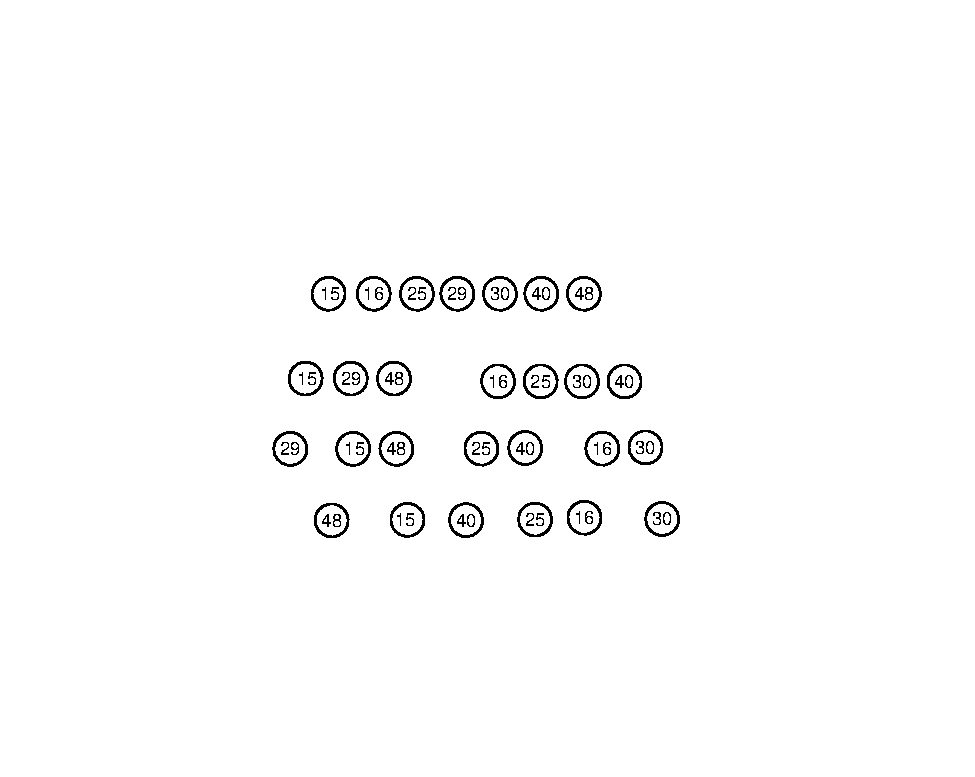
\includegraphics[width=0.5\linewidth]{2_merge}
	\caption{Merge Sort}
	\label{fig:2ms}
\end{figure}

\begin{codebox}
	\Procname{$\proc{Merge sort($A$)}$}
	\li $15, 16, 25, 29, 30, 40, 48$
	\li $15, 29, 48 || 16, 25, 30, 40$
	\li $29 || 15, 48 || 25, 40 || 16, 30$
	\li $- || 48 || 15 || 40 || 25 || 16 || 30$
\end{codebox}

\section{Question 4: CLRS Problem 2-1}
\subsection{a. show time complexity}
$\Theta(T) = \frac{n}{k}\Theta(k^{2}) = \Theta(nk)$
\subsection{b. show merge, c. show whole, max k}

There should not be anything special about Merge function, just use the original interface and implement of Merge in CLRS pp 31.\\
$$ T(n)=\left\{
\begin{array}{lcl}
 n       &      & {n \le k}\\
2T(\frac{1}{2}n) + n     &      & {n > k}\\
\end{array} \right. $$

Regarding the iterative tree, it is easy to notice that:
For branch (Merge), the complexity: $\Theta(nlg\frac{n}{k})$, For leaf (Insertion): $\Theta(nk)$, The sum is: $\Theta (nlg\frac{n}{k} + nk) $

\begin{codebox}
	\Procname{$\proc{Merge-sort-insertion($A, p, r, k$)}$}
	\li \If $r-p + 1 \le k$
	\li \Then   Insertion-Sort$(A,p,r)$
	\li 		\Return
	\li \ElseIf $p < r$
	\li \Then	$q = \left \lfloor (p+r)/2 \right \rfloor$
	\li 		Merge-Sort($A, p, q$)
	\li			Merge-Sort($A, q+1, r$)
	\li			Merge ($A, p, q, r$)
	\li			\Return
	\li \Else  \Return
	\End
\end{codebox}

Consider $\Theta (nlg\frac{n}{k} + nk) = \Theta (nlgn - nlgk + nk) = \Omega(nlgn)$, When $k = \Theta(lgn)$, it is OK.\\
But when $k = \omega(lgn), sum = \Theta(nk) = \omega(nlgn)$, so $k_{max} = \Theta(lgn)$

\subsection{d. how to choose k}
Note that in practice, we could have:\\
$T(n,k) = c_{2} (c_{1}nk + nlg(\frac{n}{k}))\\
\frac{\partial T(n,k)}{\partial k} = c_{2} (c_{1}n - \frac{n}{k})$\\
$c_{1} = \frac{constant-of-insertion-sort}{constant-of-merge-sort}$, obviously<1 according to the question\\
$k \in [0, \infty], k = \frac{1}{c_{1}} = \frac{constant-of-merge-sort}{constant-of-insertion-sort} $ could minimize T(n,k)

\section{Question 5: CLRS Problem 6.1-3}
1. Since $x.Parent.key \ge x.key$, we have:\\
When $root.child.child \neq null, root.child.key \ge root.child.child.key$\\
When $root.child.child = null$, the conclusion naturally correct\\
2. Combined with $x.key \ge x.child.key$, using deduction, it is easy to conclude that $\forall h, root.child.key \ge root.(child)^{h}.key$

\section{Question 6: CLRS Problem 6.2-6}

1. Note that the height of a Heap is no more than $lg(n+\frac{1}{2}n - 1)$ in worst condition\\
2. Note that each round of $MAX-HEAPIFY$ takes constant time\\
4. Each time $MAX-HEAPIFY$ happen, the height of pointer $\leftarrow$ pointer- 1\\
5. We have:\\ 
	$$ T(h)=\left\{
	\begin{array}{lcl}
	c       &      & {h = 0}\\
	T(h - 1) + c     &      & {n > 0}\\
	\end{array} \right. $$\\

Solves: $T(h) = \Theta(h) = \Omega((lg\frac{3}{2}n - 1) = \Omega (lgn)$

\section{Question 7: Draw Heap Sort Procedure}

Build max heap, See Figure~\ref{fig:2bh}\\
heap sort, See Figure~\ref{fig:2hs}

\begin{figure}
	\centering
	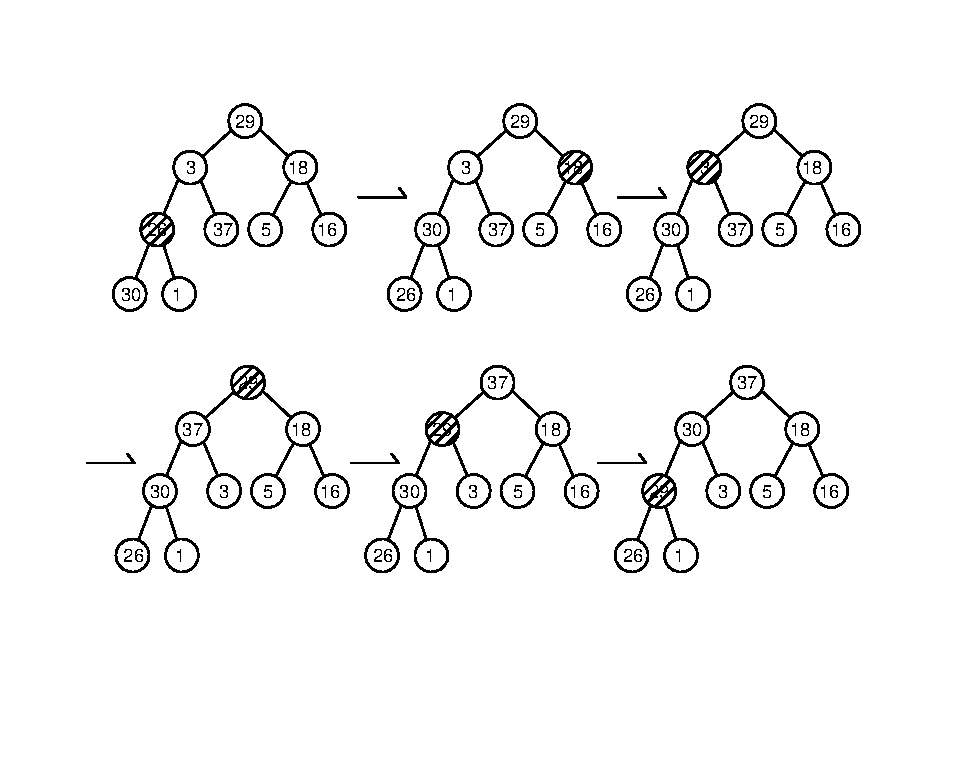
\includegraphics[width=0.9\linewidth]{2_build_heap}
	\caption{Build Heap}
	\label{fig:2bh}
\end{figure}

\begin{figure}
	\centering
	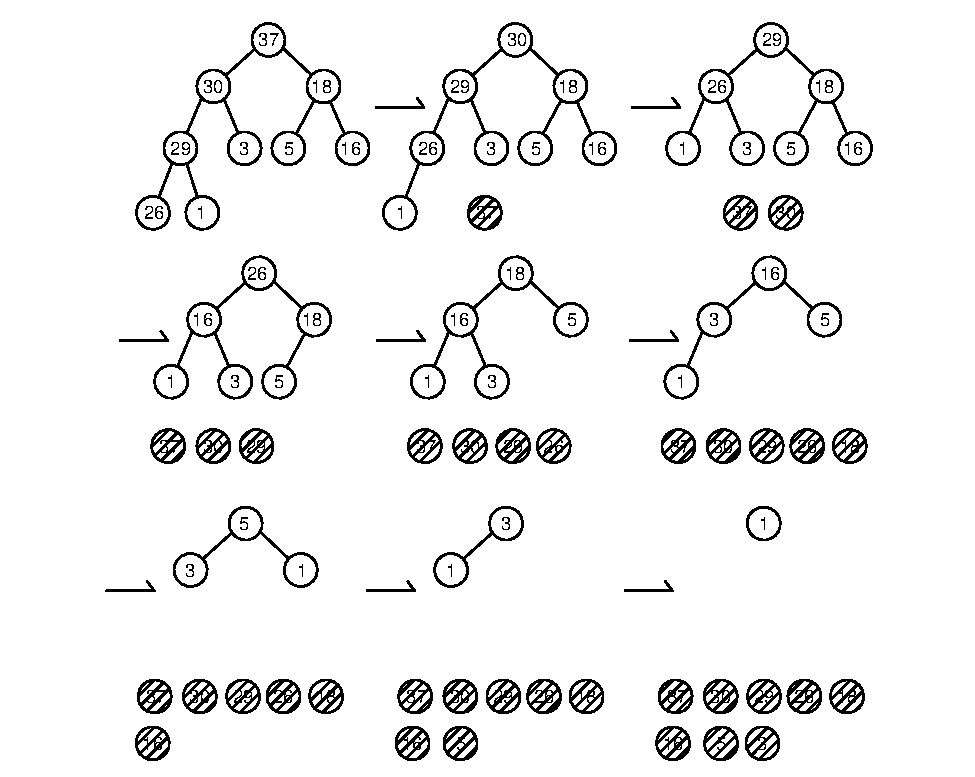
\includegraphics[width=0.9\linewidth]{2_heap_sort}
	\caption{Heap Sort}
	\label{fig:2hs}
\end{figure}

\section{Question 8: CLRS Problem 6-2}
\subsection{a. how to present}
Within a part of array A[1, n]\\
get parent, Parent[i] $ = \left \lfloor (i+d-2)/d \right \rfloor$\\
get (k+1)th child, $k \in [0, d-1]$ Child[i,k] $= di + k$\\

\subsection{b. height}
$h = \left \lfloor log_{d}n \right \rfloor $

\subsection{c. extract max}

implement of max child value and index of i in $\Theta(d)$:\\
\begin{codebox}

	\Procname{$\proc{maxChild($A, i, d$)}$}
	\li $max = -\infty$
	\li $maxIndex = -1$
	\li \For $k \gets 0$ \To $d-1$
	\li 	\Do  \If $di+k \le n=A.size()$
	\li 	\Then $max = A[di + k]>max?A[di+k]:max$
	\li			 $maxIndex =  A[di + k]>max?[di+k]:maxIndex$
	\End
	\End
	\li \Return $max, maxIndex$

\end{codebox}

implement of d-maxHeapify:\\
\begin{codebox}
	
	\Procname{$\proc{maxHeapify($A, i, d$)}$}
	\li \While $i \le n = A.size()$
	\li \Do	\If $A[i] \le maxChild(A,i,d)[0]$
	\li 		\Then $swap(A[i], maxChild(A,i,d)[1])$
	\li 		  	$i = maxChild(A,i,d)[1]$
	\End
	\End
	\li \Return
\end{codebox}

$ T(h)=\left\{
\begin{array}{lcl}
\Theta(d)       &      & {h = 0}\\
T(h-1) + \Theta(d)     &      & {h > 0}\\
\end{array} \right. $\\

From iteration tree, it is easy to find that MaxHeapify from root for d-dimension heap cost $\Theta(dlog_{d}n)$
	
\begin{codebox}
	
	\Procname{$\proc{extractMax($A,d$)}$}
	\li $max = A[1]$
	\li $swap(A[1], A[n])$
	\li $erase(A[n])$
	\li $maxHeapify(A, 1, d)$
	\li \Return $max$\\
\end{codebox}

Extract is simple, also cost  $\Theta(dlog_{d}n + Constant)$

\section{Question 9: Visualize CLRS Problem 7-1}

See Figure~\ref{fig:2hp}

\begin{figure}
	\centering
	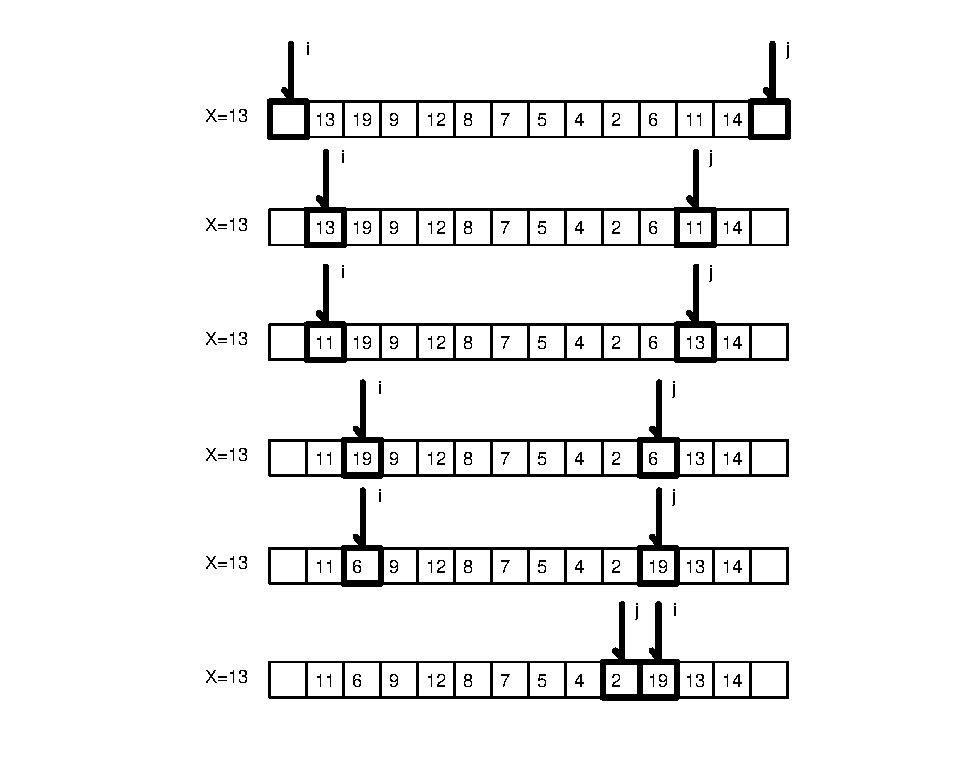
\includegraphics[width=0.9\linewidth]{2_hpar}
	\caption{Hoare partition}
	\label{fig:2hp}
\end{figure}

\end{document}
